% this is samplepaper.tex, a sample chapter demostrating the
% LLNCS macro package for Springer Computer Science proceedings;
% Version 2.20 of 2017/10/04
%
\documentclass[runningheads]{llncs}
%
\usepackage{graphicx}
\usepackage{listings}

\usepackage{subcaption}
\usepackage{array}

\usepackage[table]{xcolor}
\usepackage{multirow,bigstrut}
\usepackage{rotating}
%...

%\usepackage{siunitx} % Required for alignment

%\sisetup{
%  round-mode          = places, % Rounds numbers
%  round-precision     = 4, % to 4 places
%}

%..

% Used for displaying a sample figure. If possible, figure files should
% be included %in EPS format.
%
% If you use the hyperref package, please uncomment the following line
% to display URLs in blue roman font according to Springer's eBook style:
% \renewcommand\UrlFont{\color{blue}\rmfamily}

\begin{document}
%
\title{Fuzzy Adaptation of Parameters in a Multi-Swarm Particle Swarm Optimization (PSO) Algorithm Applied to the Optimization of a Fuzzy Controller } 

%
\titlerunning{Fuzzy Adaptation of Parameters in a MS-PSO}
% If the paper title is too long for the running head, you can set
% an abbreviated paper title here
%
\author{Alejandra Mancilla\orcidID{0000-0003-0430-8152} \and
Oscar Castillo\orcidID{0000-0002-7385-5689} \and
Mario García-Valdez\orcidID{0000-0002-2593-1114}}
%
\authorrunning{A. Mancilla et al.}
% First names are abbreviated in the running head.
% If there are more than two authors, 'et al.' is used.
%
\institute{Tijuana Institute of Technology / Tecnologico Nacional de Mexico, Tijuana, Mexico\\
    \email{\{alejandra.mancilla,mario\}@tectijuana.edu.mx,ocastillo@tectijuana.mx}}

%
\maketitle              % typeset the header of the contribution
%
\begin{abstract}

     Many control problems require running numerous simulations to find a suitable configuration for the controller's parameters. Population-based distributed algorithms can be used to speed up this procedure. One way to do this is to use multiple independent populations, each running an independent search algorithm in parallel. It is difficult to find the ideal configuration for these algorithms, such as the number of swarms, defining how particles are exchanged between swarms, and especially the parameters that affect exploration and exploitation in the search. We suggest a version of Particle Swarm Optimization (PSO) that includes a Fuzzy Inference System (FIS) to change the algorithm parameters dynamically. The adjustment considers two variables: population diversity and the number of iterations performed on the population. As an output of the FIS, we obtain the adapted parameters, representing the new values for the social and cognitive coefficients to be used in the next iteration. We aim to evaluate if this strategy helps minimize the evaluation time and minimize the root-mean-square error (RMSE). As a case study, the distributed PSO algorithm is applied to optimize the membership functions of a fuzzy controller for tracking the trajectory of an autonomous mobile robot. When compared to other configuration strategies, experimental results achieve a similar RMSE.

\keywords{Fuzzy Control \and Distributed Algorithms \and Parameter Adaptation}
\end{abstract}
%
%
\section{Introduction}

Multi-swarm optimization is a version of swarm intelligence that uses multiple sub-swarms instead of a single swarm \cite{jain2022overview}. An advantage of having multiple swarms is that it enables the parallel execution of the local PSO algorithms.
On the other hand, this approach adds new design choices not found in a single swarm implementation. For instance, each swarm can have distinct values for the parameters controlling exploration and exploitation \cite{shi2001fuzzy}. The number of particles and their initial position could be distinctly defined for each swarm (i.e., not at random).
We must also define how (and how often) these swarms communicate with each other. Communication enables a particular advantage of a multi-population design: when isolated swarms communicate or migrate certain particles between them, they prevent premature convergence to a local minimum \cite{xia2018multi}, \cite{kennedy2006swarm}. The topology of the communication channels limiting which swarms can exchange particles is also a considerable challenge \cite{miramontes2022interval}. When choosing the right configuration, designers must consider two important complementary concepts: exploitation and exploration:
\textbf{Exploitation} considers the information obtained from the best solutions found so far.  
C1 (Cognitive Coefficient) controls how much the best personal  solutions influence the swarm. 
\textbf{Exploration} helps discover unexplored regions and avoid premature convergence. 
C2 (Social Coefficient) controls how much the best global solution influences the swarm.
Achieving a balance between these two parameters is a critical problem facing most current search and optimization techniques \cite{vargas2011estrategias}. 

The proposed fuzzy strategy aims to enhance the balance between exploration and exploitation in a distributed PSO algorithm. We analyzed how two versions of a distributed parametrization strategy behave in a particular optimization problem \cite{garcia2023distributed} to evaluate if we can use this approach in future research \cite{clerc2010particle}. Our objective is to enhance the design and overall performance of the current implementation. In this work, we use a technique called Dynamic Parameter Adaptation \cite{olivas2016dynamic}. It is currently a popular method for enhancing population-based metaheuristics. The idea is to update the parameters of the algorithm while it is in execution to get better results \cite{mancilla2023optimization}. This work uses a knowledge-based system composed of fuzzy IF-THEN rules to dynamically adapt the parameters.

It is important that the solution space is explored effectively, for which it is necessary to maintain individuals with different characteristics to cover most of the search space, trying not to converge to a local optimum too early in the search. This means that we must maintain diversity in the population (Fig. \ref{fig:diversity}). Therefore, if we have a low diversity, it means that the particles are exploiting the search space. If the diversity is high, it means that the search space is being explored \cite{wang2013diversity}. A high diversity is desired in a search algorithm at the \textbf{beginning} of the run. At the same time, a low diversity is desired at the \textbf{end} of the run.

\begin{figure} [htbp]
  \centering
  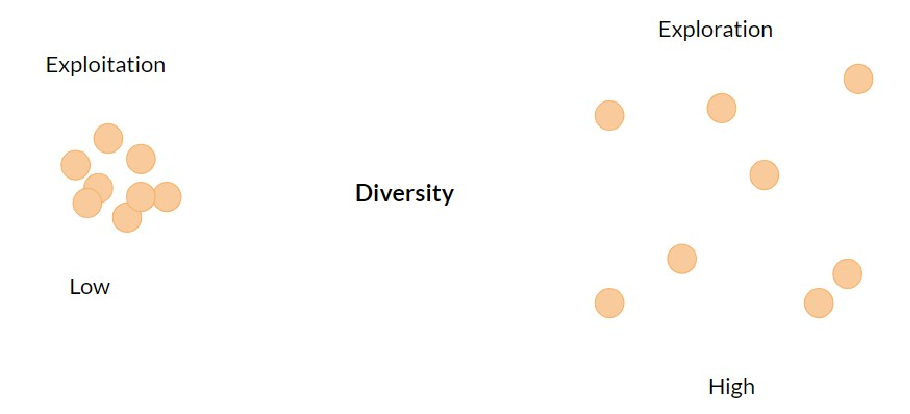
\includegraphics[angle=0,width=1\textwidth]{diversity}
  \caption{Dynamic Parameter Adaptation}
  \label{fig:diversity} 
\end{figure}

We present the results of this work as follows. In Section \ref{sec:proposal}, we discuss our proposal; Section \ref{sub:use_case} presents the experimental optimization problem, in this case, a fuzzy controller, in which we optimize the membership functions' parameters. In Section \ref{sec:results}, the experimental results are presented. The conclusions and future work are summarized in Section \ref{sec:conclusions}.

\section{Proposal}\label{sec:proposal}

For example, in a single swarm algorithm (Fig. \ref{fig:generation}). We want to have a high diversity at the beginning of the run. For example, IF Generation is LOW then C1 must be LOW while C2 is HIGH. We expect to have high diversity at the beginning of the search because each particle is created with random values, and from there, diversity begins to decrease as the algorithm advances, in which case the particles begin exploring and finish exploiting the search space \cite{cheng2011diversity}. At the beginning of the search, we want to set the cognitive coefficient (C1) to a low value and the social coefficient (C2) will be high because we want to promote exploring the search space. With this knowledge, we propose a FIS (Fig. \ref{fig:fis}), to adapt the coefficients C1 and C2 of the PSO algorithm, in which we have the number of cycles
and diversity as input variables and C1 and C2 as output variables.

\begin{figure} [htbp]
  \centering
  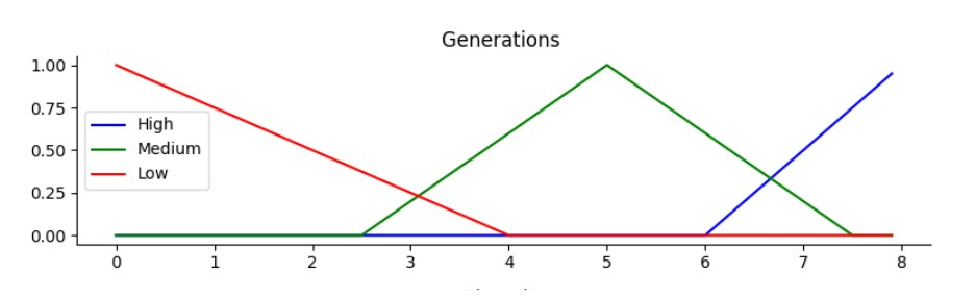
\includegraphics[angle=0,width=1\textwidth]{FM generation.pdf}
  \caption{FM's a single swarm algorithm.}
  \label{fig:generation} 
\end{figure}

\begin{figure}[htbp]
  \centering
  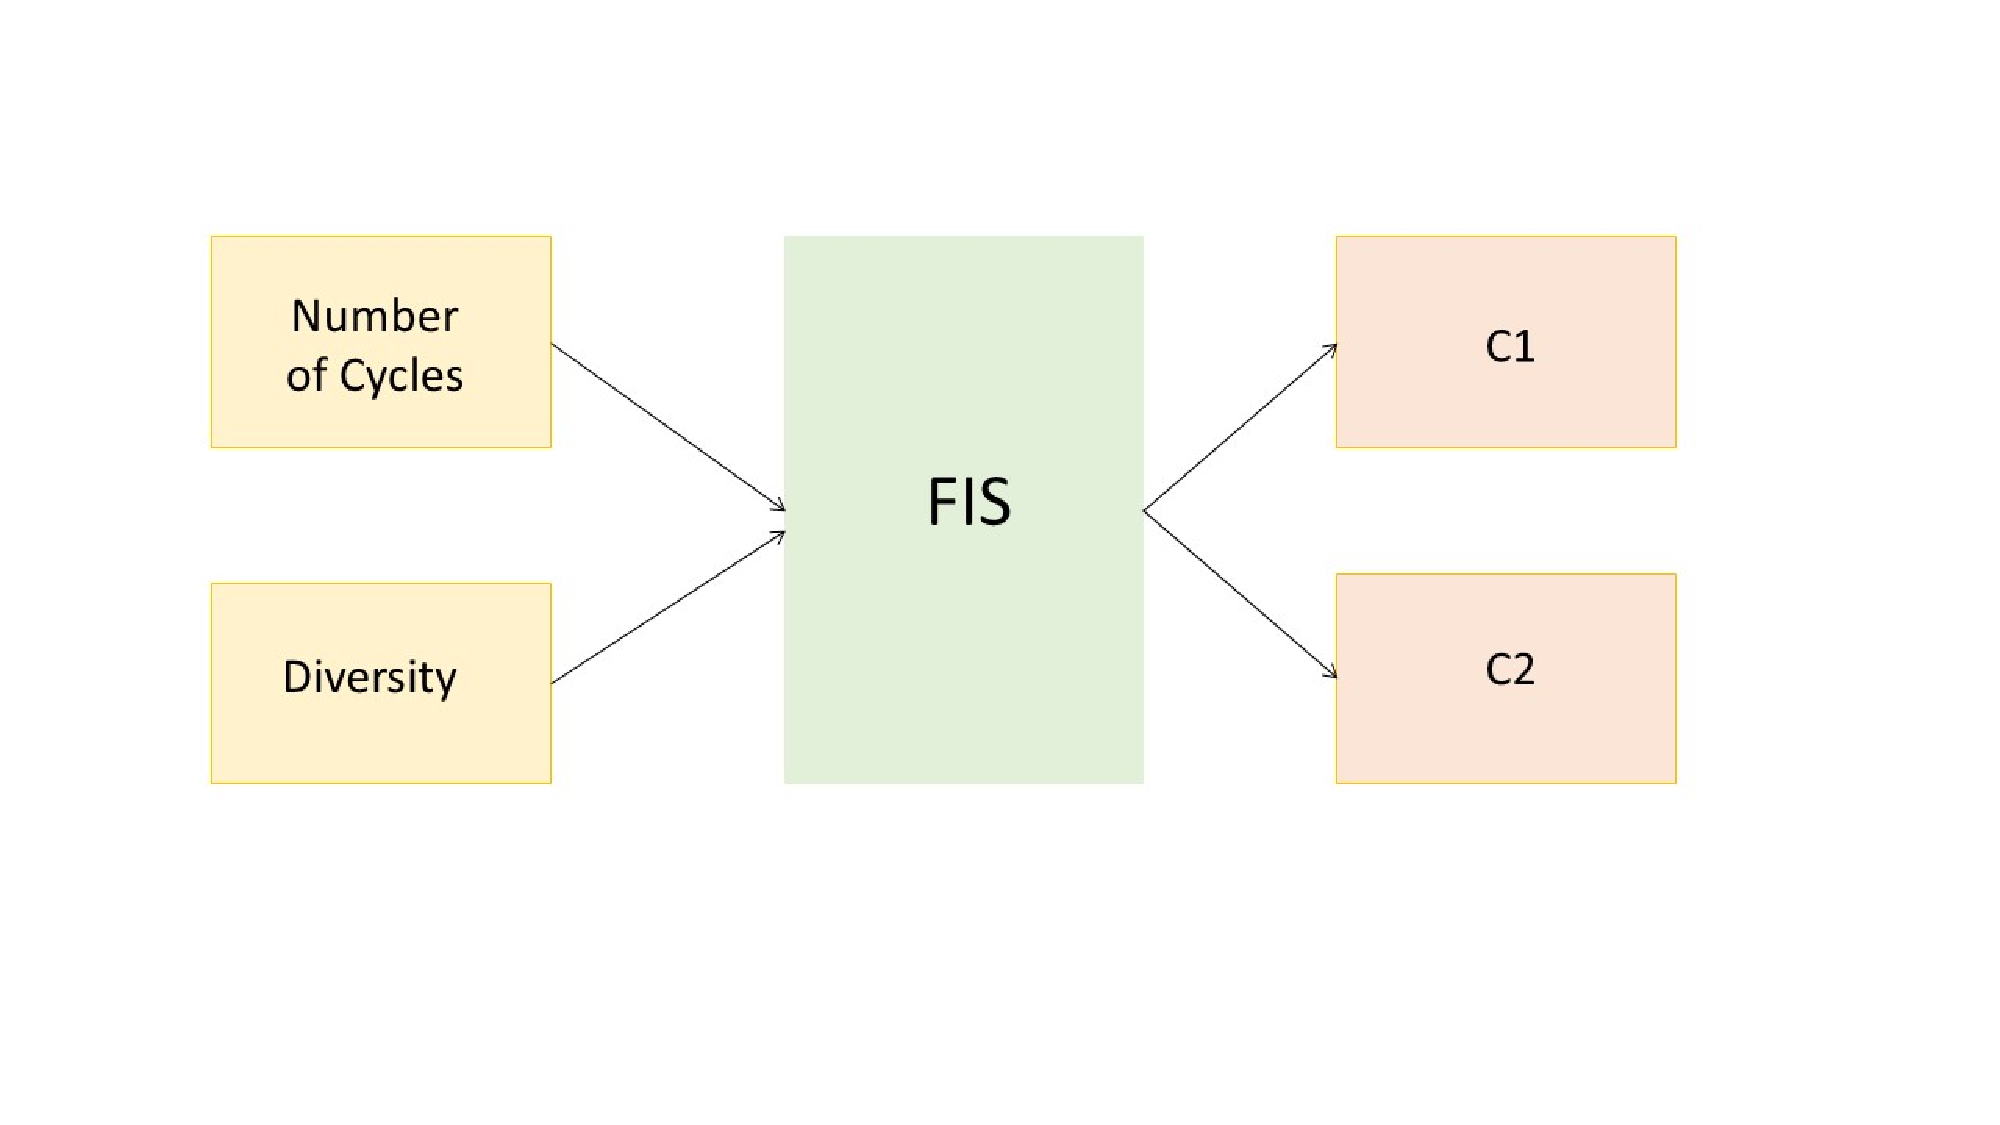
\includegraphics[angle=0,width=1\textwidth]{FIS.pdf}
  \caption{FIS for adaptation of parameters}
  \label{fig:fis} 
\end{figure}

In this Fig. \ref{fig:ejemplo}, we see an example of how diversity changes in each generation in a PSO algorithm. We measure the diversity and adjust C1 and C2 accordingly, this is done for each cycle defined in the combiner phase, in each swarm.

\begin{figure} [htbp]
  \centering
  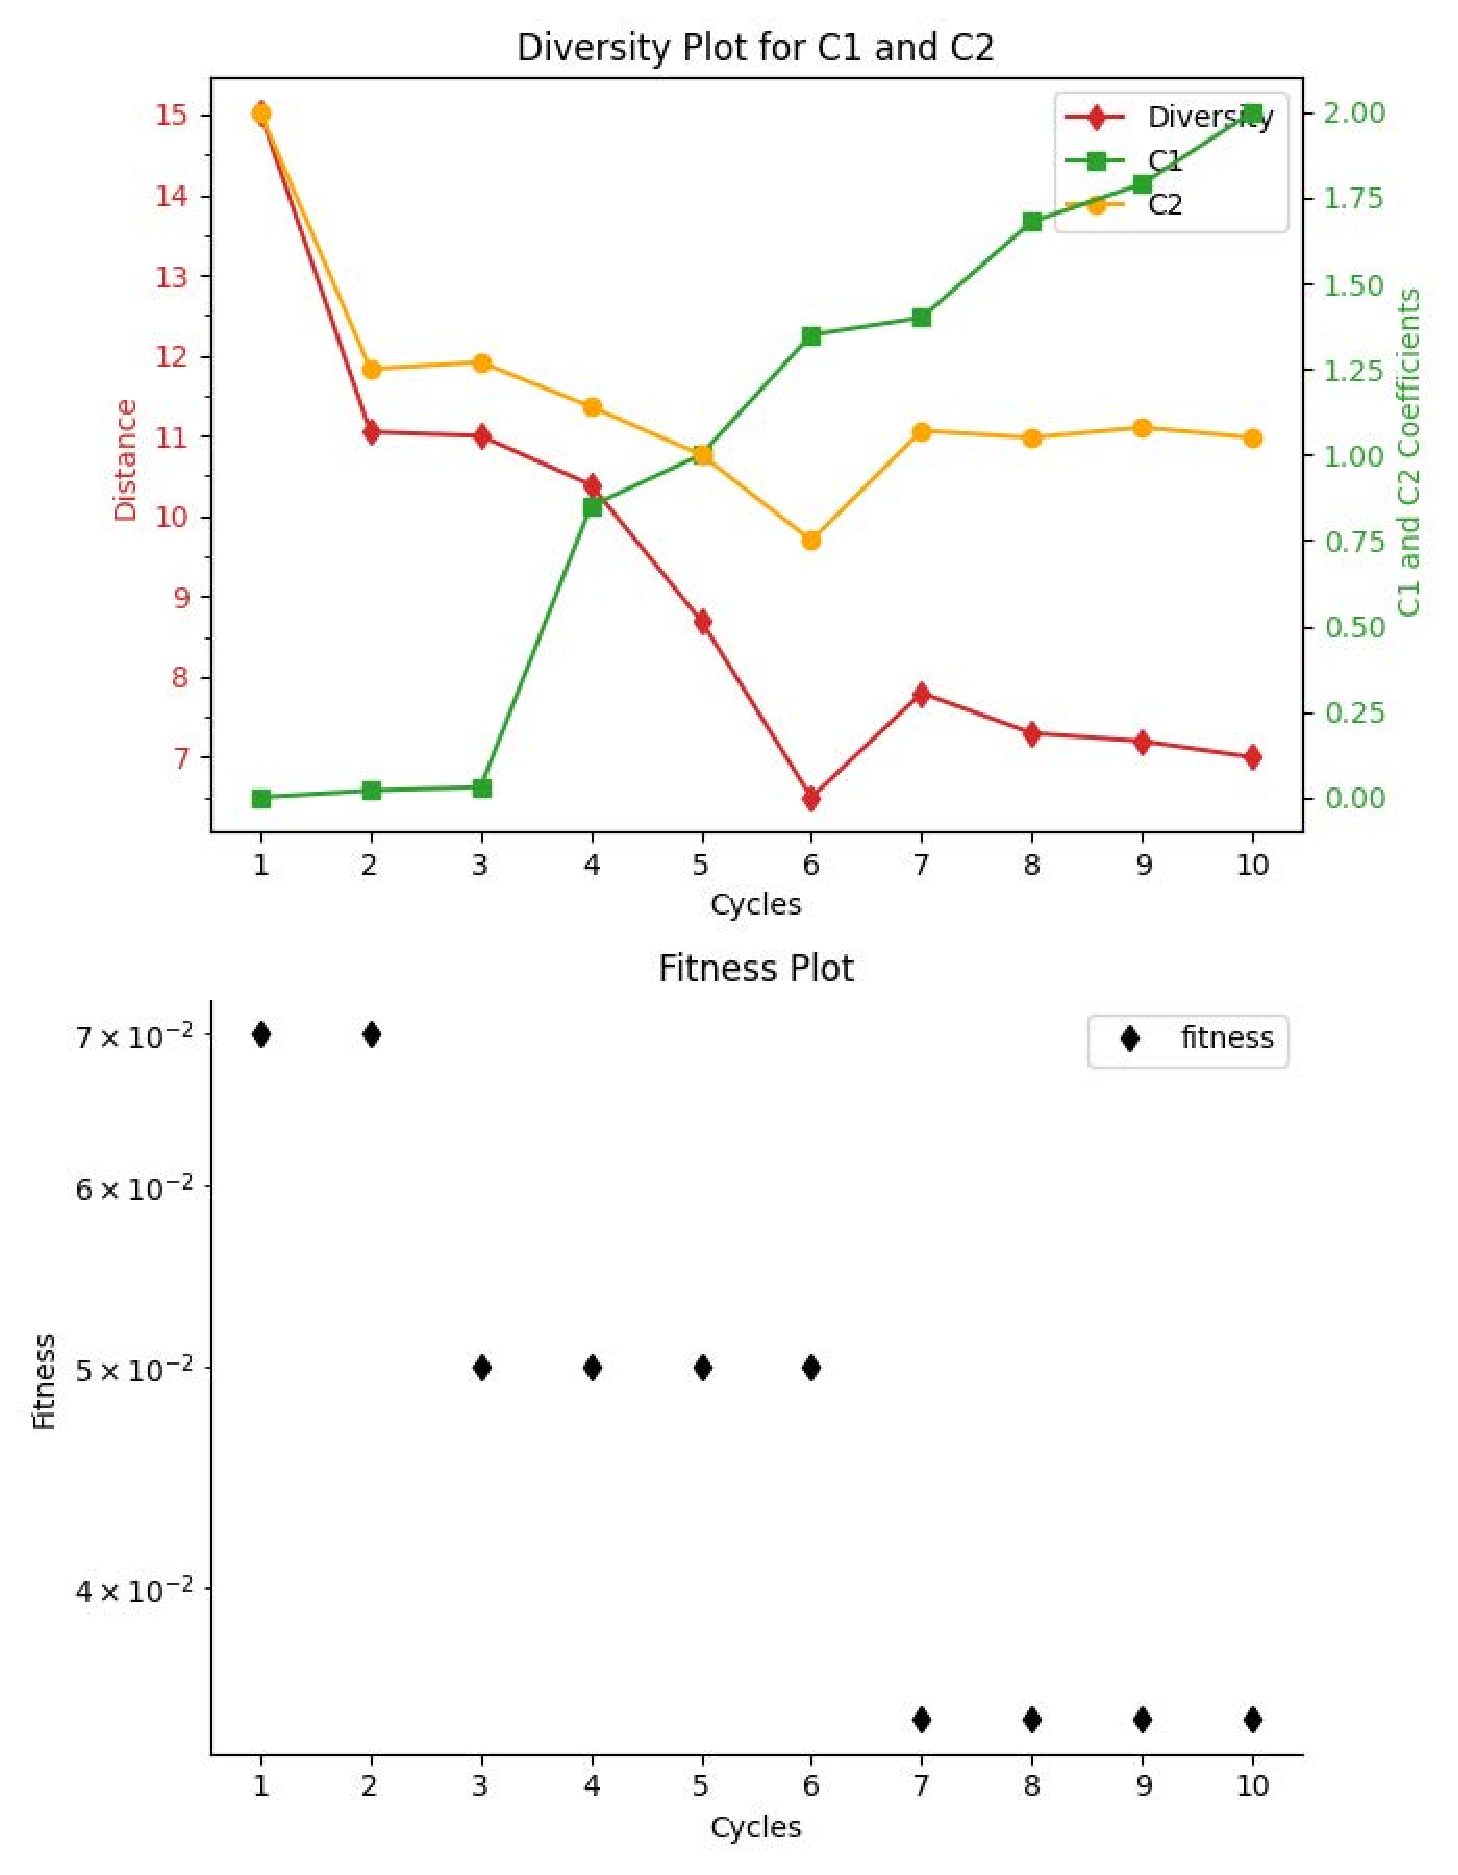
\includegraphics[angle=0,width=1\textwidth]{myplot.pdf}
  \caption{Example of changes of diversity in each cycle}
  \label{fig:ejemplo} 
\end{figure}

As we have mentioned, we can do the parameter adaptation in each iteration of the local PSO, but we can also do it in each cycle of the combiner. For our work, we experimented with both strategies and based on the results we decided to do the parameter adjustment by cycles because it gave similar results (Fig. \ref{fig:adap}).

\begin{figure}[htbp]
  \centering
  \begin{subfigure}{0.8\textwidth}
    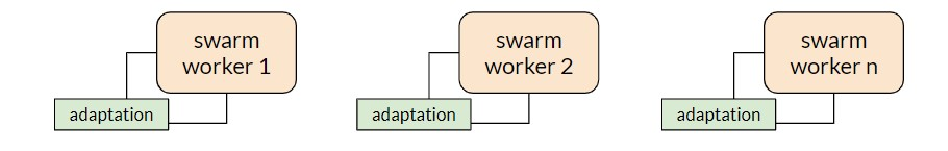
\includegraphics[angle=0,width=1\textwidth]{adaptation local.pdf}
    \caption{Adaptation can be on each iteration on the local PSO.}
    \label{fig:adap_local} 
  \end{subfigure}

  \begin{subfigure}{0.8\textwidth}
     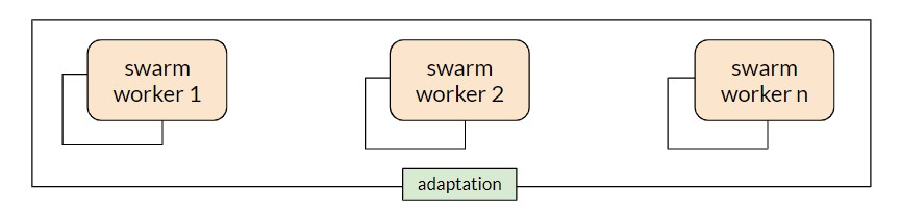
\includegraphics[angle=0,width=1\textwidth]{adaptation combiner.pdf}
     \caption{Adaptation can be done on each cycle of the combiner.}
     \label{fig:adap_combiner} 
  \end{subfigure}
\caption{Strategies for parameter adjustment.}
\label{fig:adap}
\end{figure}

Here we have the multi-swarm design, in which multiple swarms are created and added to an Input queue, multiple workers then evolve these swarms, and finally, they migrate in the combinator process. This cycle is repeated several times. The dynamic adaptation of C1 and C2 is executed each time a swarm reaches the combinator.

Figure \ref{fig:member} shows the membership functions and the relationship with the input variables diversity and cycle, and the output variables C1 and C2. After several experiments, we found that for this use case, the diversity of the swarms is less than 20 in most cases. For these experiments, we establish that ten cycles 10 of swarm combinations give the required number of function evaluations for the comparisons. Following, the convention, we set the values of C1 and C2 between 1 and 2.

\begin{figure} [htbp]
  \centering
  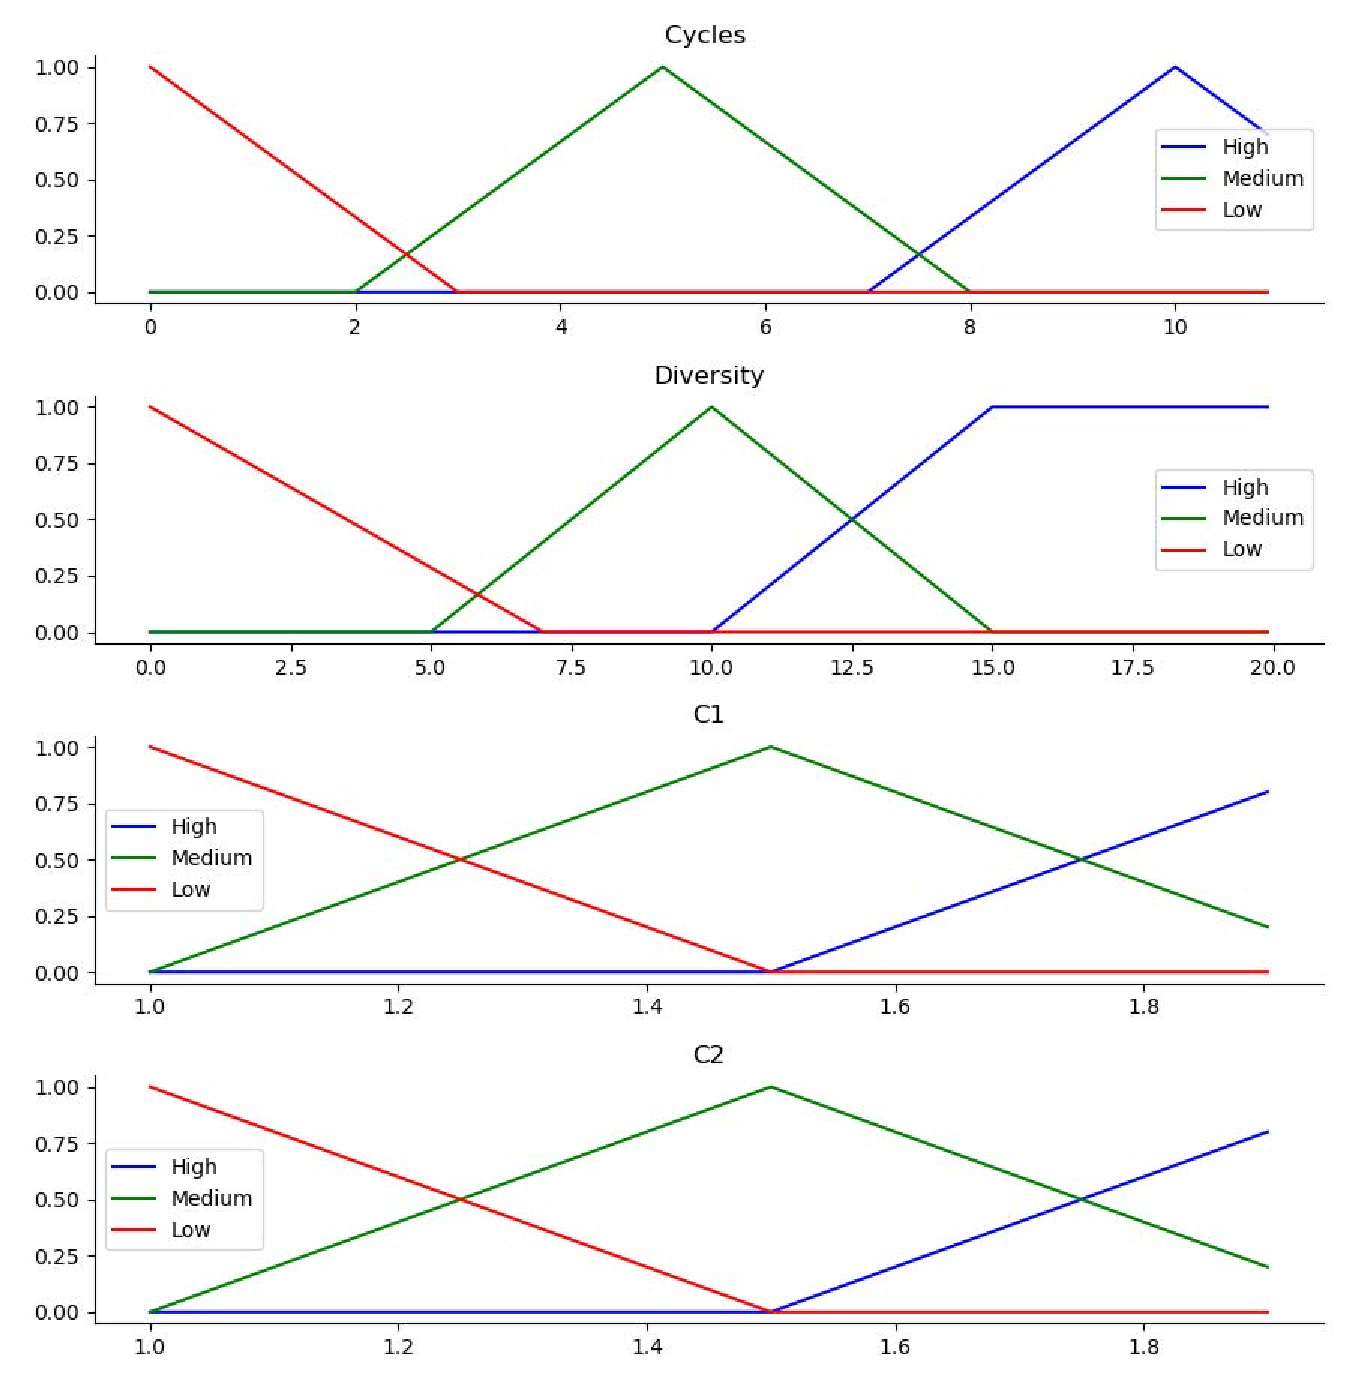
\includegraphics[angle=0,width=1\textwidth]{Figure_1.pdf}
  \caption{Membership Functions}
  \label{fig:member} 
\end{figure}

The fuzzy inference system for updating the C1 and C2 parameters has a  total of nine rules, it has two inputs: the current cycle of the algorithm and the diversity of the current swarm. The fuzzy rules are shown in Table \ref{tab:fuzzy_rules}. 

\begin{table}[htbp] 
\caption{Fuzzy Rules}\label{tab:fuzzy_rules}
\setlength{\tabcolsep}{8pt}
\begin{tabular}{l l l l l l l}
\hline
\textbf{Rule 1}  & if cycle is & hi & and diversity is & hi & then C1 is & hi  \\
                 &             &    &                  &    & and C2 is  & low \\ \hline
\textbf{Rule 2}  & if cycle is & hi & and diversity is & med & then C1 is & hi  \\
                 &             &    &                  &    & and C2 is  & med \\ \hline
\textbf{Rule 3}  & if cycle is & hi & and diversity is & low & then C1 is & hi  \\
                 &             &    &                  &    & and C2 is  & low \\ \hline
\textbf{Rule 4}  & if cycle is & med & and diversity is & hi & then C1 is & med  \\
                 &             &    &                  &    & and C2 is  & hi \\ \hline
\textbf{Rule 5}  & if cycle is & med & and diversity is & med & then C1 is & med  \\
                 &             &    &                  &    & and C2 is  & med \\ \hline
\textbf{Rule 6}  & if cycle is & med & and diversity is & low & then C1 is & med  \\
                 &             &    &                  &    & and C2 is  & low \\ \hline
\textbf{Rule 7}  & if cycle is & low & and diversity is & hi & then C1 is & low  \\
                 &             &    &                  &    & and C2 is  & hi \\ \hline
\textbf{Rule 8}  & if cycle is & low & and diversity is & med & then C1 is & low  \\
                 &             &    &                  &    & and C2 is  & med \\ \hline
\textbf{Rule 9}  & if cycle is & low & and diversity is & low & then C1 is & low  \\
                 &             &    &                  &    & and C2 is  & hi \\ \hline

\end{tabular}
\end{table}

\subsection{Use Case}\label{sub:use_case}

We optimize the membership functions for a benchmark control problem. A rear-wheel controller \cite{paden_survey_2016}. The parameters of the multi-swarm version of the PSO algorithm are shown in Table  \ref{tab:alg_params}.
The multi-swarm is composed of sixteen swarms with ten particles each. Each local PSO will run for eight iterations of the algorithm before returning the resulting swarm state to the output queue. All swarms will complete ten cycles, meaning they will go through the combiner and back to the input queue a total of ten times each.


\begin{table}[htbp] 
\caption{Experimental Setup}\label{tab:alg_params}
\setlength{\tabcolsep}{10pt}
\begin{tabular}{l l l}
\hline
\textbf{Algorithm} & \textbf{Parameter}	& \textbf{Range [min,max]}\\ \hline
MS-PSO & Communication Topology & Fully connected  \\
& Speed.       & Min=[-0.20, -0.30] \\
&              & Max=[0.20, 0.30]  \\
& Cognitive and Social $C_1,C_2$ &  [1.0, 2.0]  \\ \hline
Swarms      & Swarm Size              & 10  \\
            & Number of Swarms        & 16 \\
            & Number of Iterations    &  8 \\
            & Number of Cycles        & 10   \\
            & Dimension.              & 15   \\   
            & \#Funcion Evaluations           & 12800 \\ \hline
\end{tabular}
\end{table}

\section{Results}\label{sec:results}

In Table \ref{tab:rmse}, we show the results of the experiments. The distributed results with parameters with dynamically adjusted values are compared against a distributed version initialized with random parameters for each swarm; this is found in our previous work.

We establish that on average, the multi-swarm PSO using dynamic parameter adaptation yields better results than the distributed heterogeneous parameters variant. Table \ref{tab:rmse} shows the average RMSE obtained in thirty runs.


\begin{table}[htbp]
    \caption{average RMSE obtained in thirty runs.} 
    \label{tab:rmse}
    \centering
    \setlength{\tabcolsep}{8pt}
    \begin{tabular}{|c|c|c|}      \hline
      \multicolumn{3}{|c|}{RMSE} \\ \hline
      & {Heterogeneous Parameters}  & {  Dynamic Parameter Adaptation} \\ \hline
    AVERAGE   & 0.00305315 & 0.00284276 \\ \hline
    STDDEV    & 0.00080043 & 0.00064820 \\ \hline   
    MEDIAN    & 0.00290360 & 0.00271963 \\ \hline 
    MIN       & 0.00127626 & 0.00168746 \\ \hline   
    MAX       & 0.00496247 & 0.00448633 \\ \hline    
   \end{tabular}
\end{table}

A statistical test Z (see Table \ref{tab:ztest}), compared the same algorithms using heterogeneous parameters and the algorithms with dynamic adaptation of parameters, the test concluded that there is not enough evidence to reject the null hypothesis, because the p-value is not within the acceptable confidence interval.

\begin{table}[htbp] 
  \caption{Z test.}
  \label{tab:ztest}
  \centering
  \setlength{\tabcolsep}{5pt}
  \begin{tabular}{|c|c|c|}  
  \hline
    \multicolumn{3}{|c|}{  p-values, $\alpha$=0.05, 30 independent samples,  unequal variances.}  \\ [1ex] \hline
    $H_a$ : $\mu_{eAi}$ $>$ $\mu_{eAj}$ &  Heterogeneous  & Dynamic Parameter   \\   
                                        & Parameters      &  Adaptation  \\   \hline
            Heterogeneous Parameters    & \cellcolor{lightgray}    & 0.8659  \\  \hline
         Dynamic Parameter Adaptation   &   0.1341  & \cellcolor{lightgray} \\ \hline    
  \end{tabular}
\end{table}

 Figure \ref{fig:boxplot} shows the same results using a box plot. Again, there is no difference between the median of both algorithms.

\begin{figure}[htbp]
  \centering
  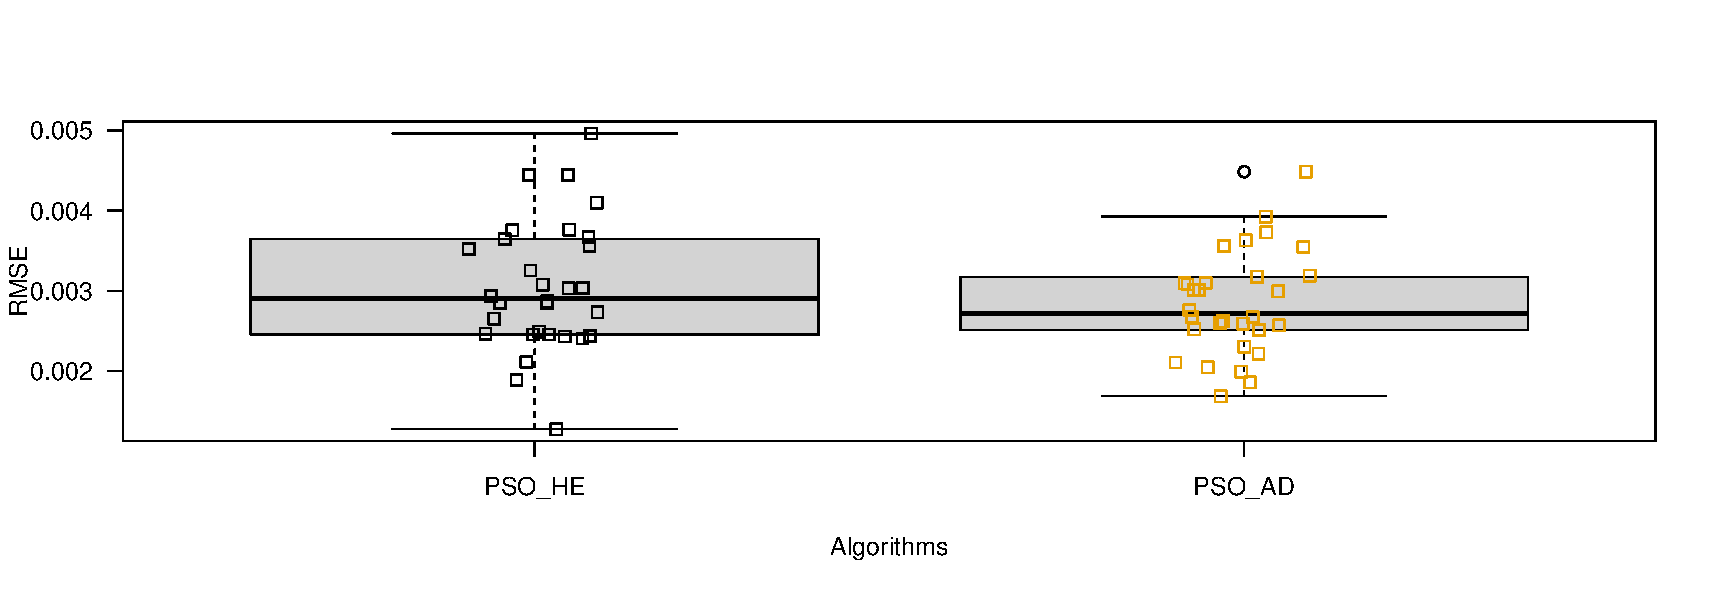
\includegraphics[angle=0,width=1\textwidth]{RplotAjusteParam.pdf}
  \caption{Box-plot of the data.}
  \label{fig:boxplot} 
\end{figure}

\section{Conclusions and Future Work}\label{sec:conclusions}

We presented a dynamic adaptation technique based on fuzzy logic, applied to a distributed multi-swarm PSO algorithm method. We then applied the proposed system to the optimization problem of tuning the parameters defining the MFs of a fuzzy controller. To validate the proposal, we conducted an experiment comparing two strategies: fuzzy adaptation and heterogeneous configurations of the algorithms. We found that both strategies yield similar results. The adaptation of parameters could be further studied, to see if other metrics can be considered to determine the balance between the exploration and exploitation of the search space. Moreover, other parameters found in a multi-swarm design could have a greater impact. For instance, the number of particles exchanged between swarms could be adapted to promote or limit the overall diversity.

\begin{acknowledgement}
    This work is financed in part by Project 18186.23-P of 2021 TecNM research grants.
\end{acknowledgement}

%
% ---- Bibliography ----
%
% BibTeX users should specify bibliography style 'splncs04'.
% References will then be sorted and formatted in the correct style.
%
\bibliographystyle{splncs03_unsrt}
\bibliography{biblio}
%
%\begin{thebibliography}{8}

%\end{thebibliography}
\end{document}

